\documentclass[english]{article}
\usepackage{tikz}
\usepackage{pgfplots}
\pgfplotsset{compat=1.10}
\usetikzlibrary{shapes.geometric,arrows,fit,matrix,positioning}
\tikzset
{
    treenode/.style = {circle, draw=black, align=center, minimum size=1cm},
    subtree/.style  = {isosceles triangle, draw=black, align=center, minimum height=0.5cm, minimum width=1cm, shape border rotate=90, anchor=north}
}
\usepackage[letterpaper]{geometry}
\geometry{verbose,tmargin=1in,bmargin=1in,lmargin=1in,rmargin=1in}
\usepackage{babel}
\usepackage{amsmath}
\usepackage{amssymb}
\usepackage{capt-of}
\usepackage{graphicx}
\usepackage{color}
\usepackage{latexsym}
\usepackage{xspace}
\usepackage{pdflscape}
\usepackage[hyphens]{url}
\usepackage[colorlinks]{hyperref}
\usepackage{enumerate}
\usepackage{ifthen}
\usepackage{float}
\usepackage{array}
\usepackage{tikz}
\usepackage{multirow} 
\usetikzlibrary{shapes}
\usepackage{algorithm2e}
\usepackage{listings}
\usepackage{diagbox}

%%%% CUSTOM MATH GOES HERE
\newcommand{\ind}[1]{\mathbf{1}\left(#1\right)}
\renewcommand{\Pr}{\mathbf{Pr}\xspace}
\newcommand{\Bern}{\textsf{Bernoulli}\xspace}
\newcommand{\sign}{\textsf{sign}}
\newcommand{\E}{\mathbf{E}}
\newcommand{\bx}{\mathbf{x}}
\newcommand{\bX}{\mathbf{X}}
\newcommand{\by}{\mathbf{y}}
\newcommand{\bY}{\mathbf{Y}}
\newcommand{\bz}{\mathbf{z}}
\newcommand{\bw}{\mathbf{w}}
\newcommand{\bl}{\mathbf{\ell}}
\newcommand{\vc}[1]{\mathbf{#1}}
\newcommand{\Hypo}{\mathcal{H}}
\newcommand{\XX}{\mathcal{X}}
\newcommand{\cD}{\mathcal{D}}
\newcommand{\argmax}{\operatornamewithlimits{argmax}}
\newcommand{\argmin}{\operatornamewithlimits{argmin}}
\newcolumntype{M}{>{$\vcenter\bgroup\hbox\bgroup}c<{\egroup\egroup$}}
\newcolumntype{x}[1]{>{\centering\arraybackslash}m{#1}}

%%%%%%%%%%%%%%%%%%%%%%%%%%%%%%%%%
\title{CIS 520, Machine Learning, Fall 2018: Assignment 5\\}
\date{}
\author{Wentao He}

\begin{document}
\maketitle
{\normalsize Collaborator: \underline{N/A}}


\section{Multiclass Boosting}
\begin{enumerate}
    \item Proof:
    \begin{align*}
    D_{T+1}(i) = &\; \dfrac{D_t(i)e^{-\alpha_t \times \hat{h}_{t, y_i}(x_i)}}{Z_T}\\
    = &\; \dfrac{D_{t-1}(i)e^{-\alpha_{t-1}\times \hat{h}_{t-1, y_i}(x_i)-\alpha_t\times \hat{h}_{T, y_i}(x_i)}}{Z_{T-1}Z_T}\\
    = &\; \dfrac{D_1(i)e^{\sum_{t=1}^{T} -\alpha_t \times \hat{h}_{t, y_i}(x_i)}}{\prod_{t=1}^{T}Z_t}\\
    = &\; \dfrac{\dfrac{1}{m}e^{-F_{T, y_i}(x_i)}}{\prod_{t=1}^{T}Z_t}
    \end{align*}
    \clearpage
    \item Proof:\\\\
    Let us first consider the case $H(x_i) = y_i$. Then both \textbf{1}$(H(x_i) \neq y_i) = 0$ and the inequality trivially hold. Then let us consider the case $H(x_i) \neq y_i$. Then we should be able to clain that $F_{T, y_i}(x_i)<0$ holds true, because if $F_{T, y_i}(x_i)>0$, then we will get $F_{T, y_i}(x_i) > F_{T,k}(x_i)$ for all $k \neq y_i$. Otherwise we will get$ \sum_{k=1}^{K} F_{T,k}(x_i) > -(K-2)\sum_{t=1}^{T} \alpha_t$, which will then lead to $H(x_i) = y_i$ and contradict our assumption in this particular problem. The inequality holds because both sides of the inequality will be 1, $\Rightarrow 1\leq 1$ holds. Therefore in conclusion, \textbf{1}$(H(x_i) \neq y_i) \leq$\textbf{ 1}$(F_{T, y_i}(x_i)\leq 0)$.
    \clearpage
    \item Proof:
    \begin{align*}
    er_S [H] = &\; \dfrac{1}{m}\sum_{i=1}^{m}\mathbf{1}(H(x_1)\neq y_1)\\
    \leq &\; \dfrac{1}{m}\sum_{i=1}^{m}\mathbf{1}(F_{T, y_i}(x_i)<0)\\
    \leq &\; \dfrac{1}{m}\sum_{i=1}^{m} e^{F_{T, y_i}(x_i)}\\
    \text{since } Z_t = &\; \sum_{j=1}^{m}D_t(j)e^{-\alpha_t\times h_{t, y_i}(x_i)} \text{ and } \sum_{i}D_{t+1}(i) = 1\\
    er_S[H] \leq &\; \dfrac{1}{m}\sum_{i=1}^{m} e^{F_{T, y_i}(x_i)} = (\prod_{t=1}^{T}Z_t)\times(\sum_{i}D_{t+1}(i)) = \prod_{t=1}^{T}Z_t
    \end{align*}
    \clearpage
    \item Proof:
    \begin{align*}
    Z_t = &\; \sum_{i=1}^{m}D_t(j)e^{-\alpha_t\times \hat{h}_{t, y_i}(x_i)}\\
    = &\; \sum_{i=1}^{m}D_t(i)e^{-\alpha_t}\mathbf{1}(H(x_i)=y_i) + \sum_{i=1}^{m}D_t(i)e^{\alpha_t}\mathbf{1}(H(x_i)\neq y_i)\\
    = &\; \sum_{i=1}^{m}D_t(i)e^{-\alpha_t}(1-\mathbf{1}(H(x_i)\neq y_i)) + \sum_{i=1}^{m}D_t(i)e^{\alpha_t}\mathbf{1}(H(x_i)\neq y_i)\\
    = &\; (\sum_{i=1}^{m}D_t(i)-\sum_{i=1}^{m}D_t(i)\mathbf{1}(H(x_i)\neq y_i)e^{-\alpha_t} +\sum_{i=1}^{m}D_t(i)e^{\alpha_t}\mathbf{1}(H(x_i)\neq y_i)\\
    = &\; (1-er_t)e^{-\alpha_t}+er_t e^{\alpha_t}\\
    \text{since }e^{\alpha_t} = &\; e^{\frac{1}{2}\ln{\frac{1-er_t}{er_t}}} = \sqrt{\dfrac{1-er_t}{er_t}}\\
    \text{so } Z_t = &\; 2 \times \sqrt{er_t(1-er_t)}
    \end{align*}
    \clearpage
    \item Proof:
    Since $er_t \leq \dfrac{1}{2} - \gamma$ for all $t$, we can choose $max(er_t) = \dfrac{1}{2}$ to prove the statement.
    \begin{align*}
    er_S [H] \leq &\; \prod_{t=1}^{T}Z_t\\
    = &\; \prod_{t=1}^{T} 2 \times \sqrt{er_t(1-er_t)}\\
    = &\; 2^T \sqrt{(\dfrac{1}{2}-\gamma)(\dfrac{1}{2}+\gamma)}^T\\
    = &\; (1-4\gamma)^{\dfrac{1}{2}T}\\
    \leq &\; e^{-2\gamma^2T}
    \end{align*}
\end{enumerate}
\clearpage
\section{Perceptron vs. Winnow}
\begin{enumerate}
    \item For perceptron:\\
    $||u||_2 = \sqrt{k}$, $R_2 = \sqrt{d}$\\
    Number of mistakes $\leq \dfrac{R_2^2 \cdot ||u||_2^2}{\gamma^2} = \dfrac{kd}{\gamma^2}$\\
    For Winnow:\\
    $||u||_1 = k$, $R_\infty = 1$\\
    Number of mistakes $\leq \dfrac{R_\infty^2 \cdot ||u||_1^2}{\gamma^2} \ln{(d)}= \dfrac{2d^2}{\gamma^2\ln{(d)}}$\\
    Therefore Winnow is a better choice.
    \clearpage
    \item Similar to the previous problem, for perceptron:\\
    $||u||_2 \leq 2\sqrt{d}$, $R_2 = \sqrt{k}$\\
    Number of mistakes $\leq \dfrac{4kd}{\gamma^2}$\\
    For Winnow:\\
    $||u||_1 = d$, $R_\infty = 1$\\
    Number of mistakes $\leq \dfrac{2d^2}{\gamma^2\ln{(d)}}$\\
    Therefore Perceptron is a better choice.
    \clearpage
    \item No. Winnow is maintaining a non-negative weight vector so it will have a non-negative dot product with all feature vectors in this particular case. Therefore Winnow will predict every label as positive, namely $>0$.
\end{enumerate}
\clearpage
 \section{Principal Component Analysis}
 \begin{enumerate}
    \item Resulting Image, please see Figure \ref{fig:3a}.\\
    \begin{figure}[H]
          \centering
          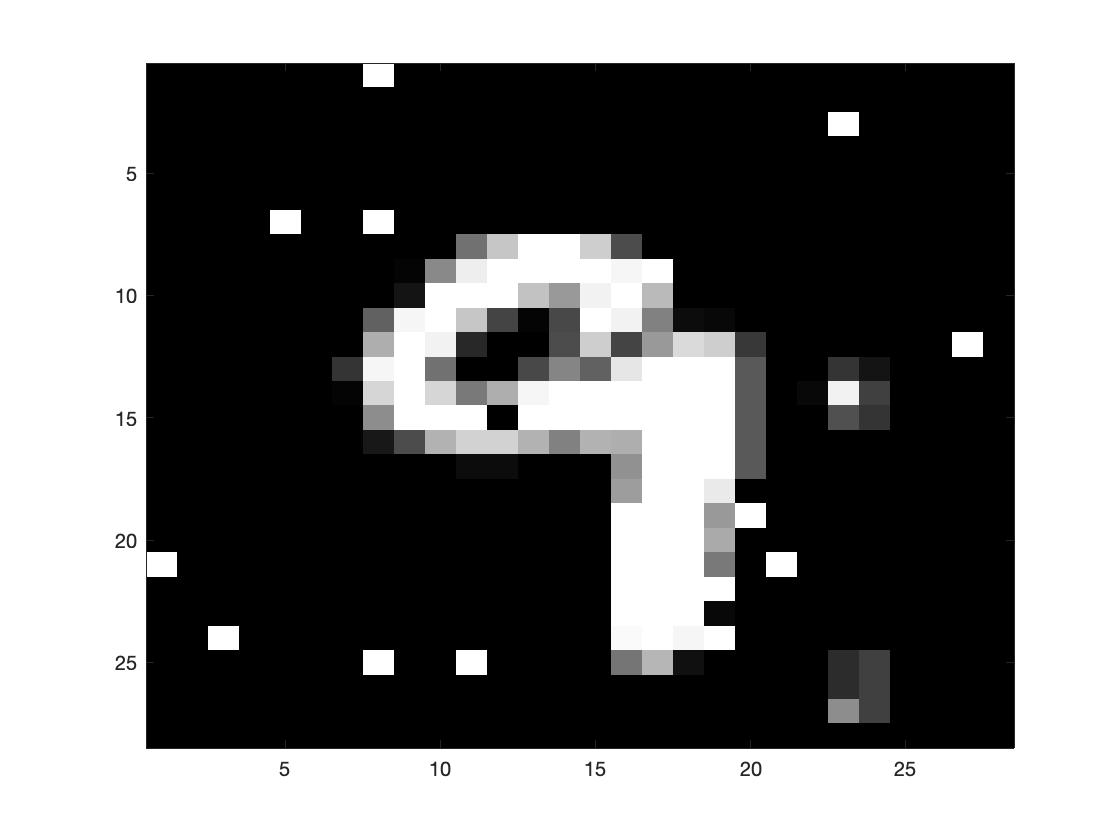
\includegraphics[width=0.7\textwidth]{3a.jpg}
          \caption{Resulting Image 1.}
          \label{fig:3a}
        \end{figure}
        Code:
        \begin{verbatim}
load('MNIST_train.mat')
last=X_train(12000,:);
last_ex=reshape(last,[28 28]);
imagesc(last_ex')
colormap('gray')
        \end{verbatim}
        \clearpage
    \item Resulting Images, please see Figure \ref{fig:3b1}, Figure \ref{fig:3b2} and Figure \ref{fig:3b3}.
    \begin{figure}[H]
          \centering
          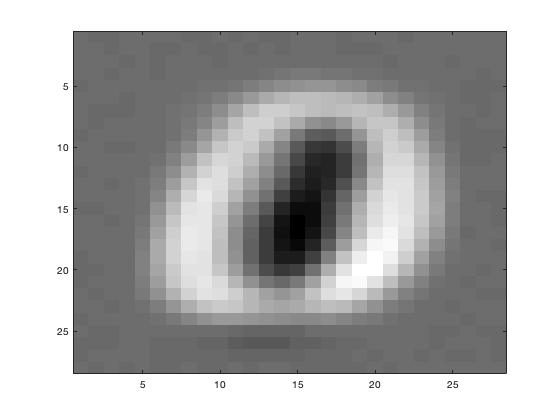
\includegraphics[width=0.7\textwidth]{3b1.jpg}
          \caption{Resulting Image 1.}
          \label{fig:3b1}
        \end{figure}
        \begin{figure}[H]
          \centering
          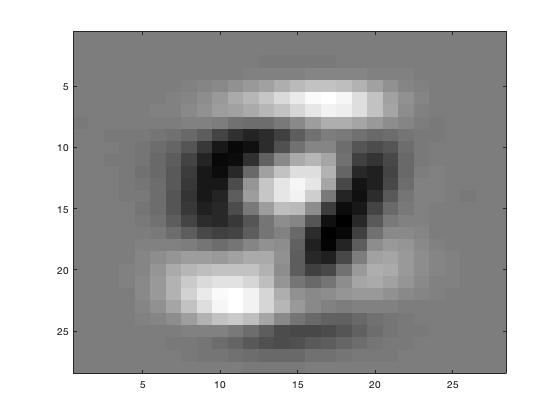
\includegraphics[width=0.7\textwidth]{3b2.jpg}
          \caption{Resulting Image 2.}
          \label{fig:3b2}
        \end{figure}
        \begin{figure}[H]
          \centering
          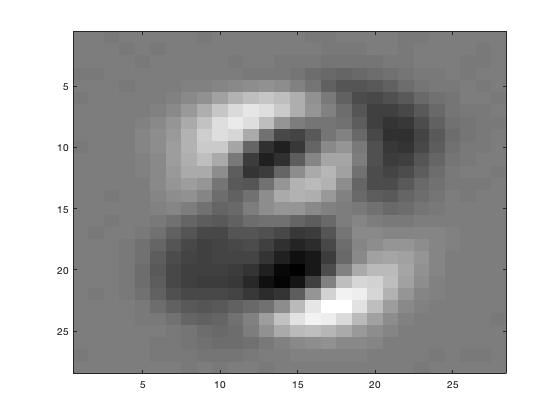
\includegraphics[width=0.7\textwidth]{3b3.jpg}
          \caption{Resulting Image 3.}
          \label{fig:3b3}
        \end{figure}
        These images make sense because the first principal component is the best straight line you can fit to the data and it has more information than others. Namely, the first principal component vector will tell you the most about the point cloud after projecting all points onto the vector.
        \clearpage
    \item For $1^{st}$ and $2^{nd}$ PC, please see Figure \ref{fig:3c1}. For $100^th$ and $101^st$ PC, please see Figure \ref{fig:3c2}.
    \begin{figure}[H]
          \centering
          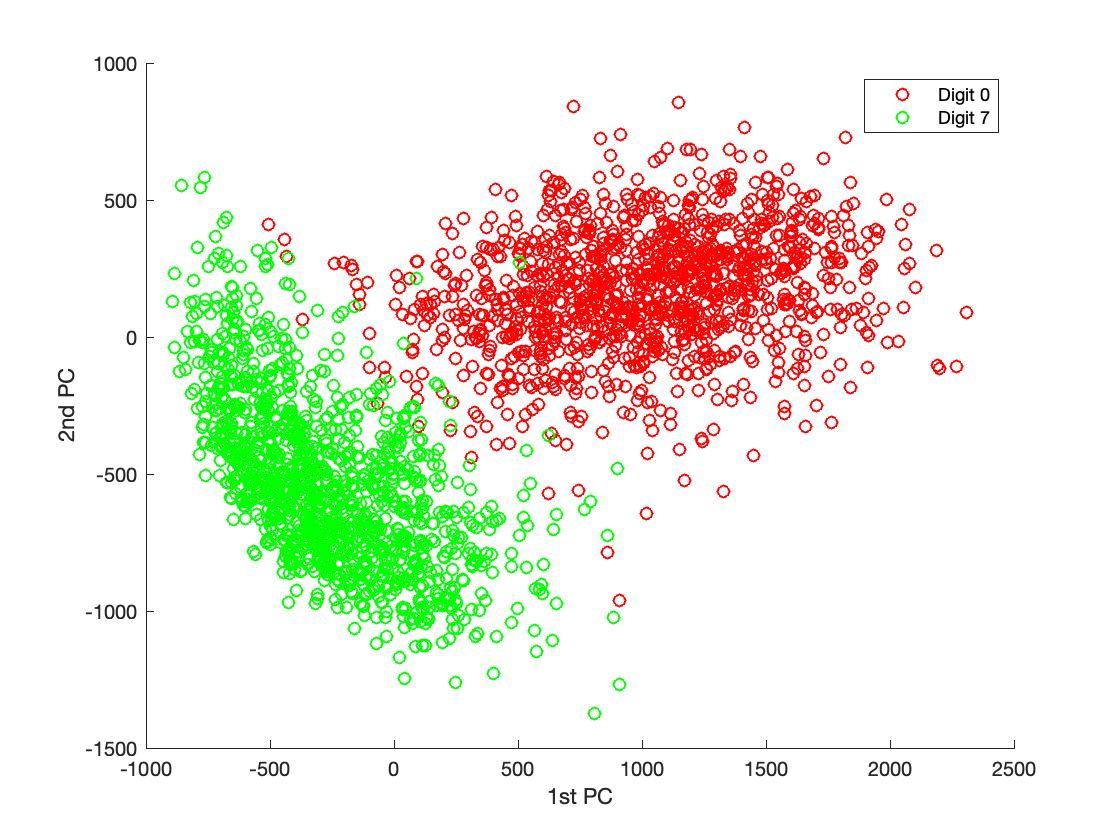
\includegraphics[width=0.7\textwidth]{3c1.jpg}
          \caption{$1^{st}$ and $2^{nd}$ PC.}
          \label{fig:3c1}
        \end{figure}
        \begin{figure}[H]
          \centering
          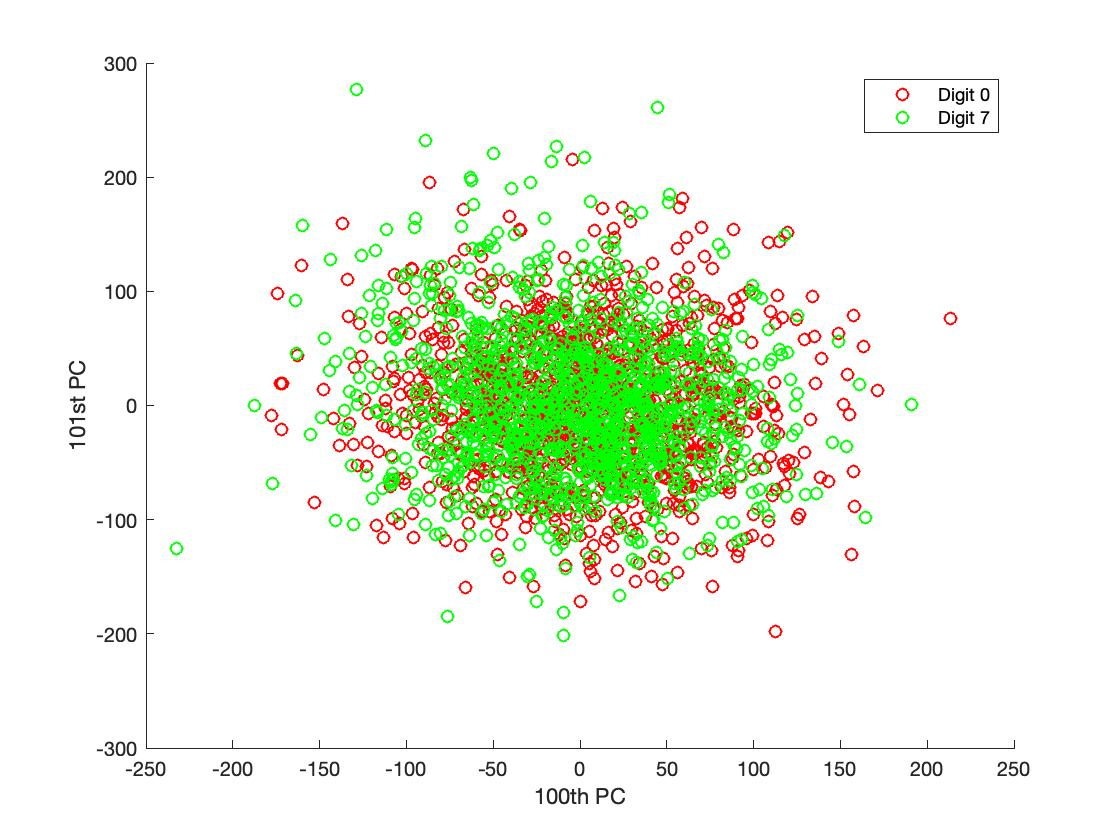
\includegraphics[width=0.7\textwidth]{3c2.jpg}
          \caption{$100^{th}$ and $101^{st}$ PC.}
          \label{fig:3c2}
        \end{figure}
        What we can observe from those two graphs is that for the 1st and 2nd PC dimensions, images are separated pretty well simply because the first two PC dimensions contain more information regarding the characters of the images, namely the difference between the 0 and the 7 characters that are contained in the first two PC dimensions. Since the first principal component vector will tell you the most about the point cloud after projecting all points onto the vector, in the second graph, 100th and 101st PC dimensions contain much more noice and less useful information regarding the differences between those two characters, so the graph is not very separated.
        \clearpage
    \item Please see Figure \ref{fig:3d1}.
    \begin{figure}[H]
          \centering
          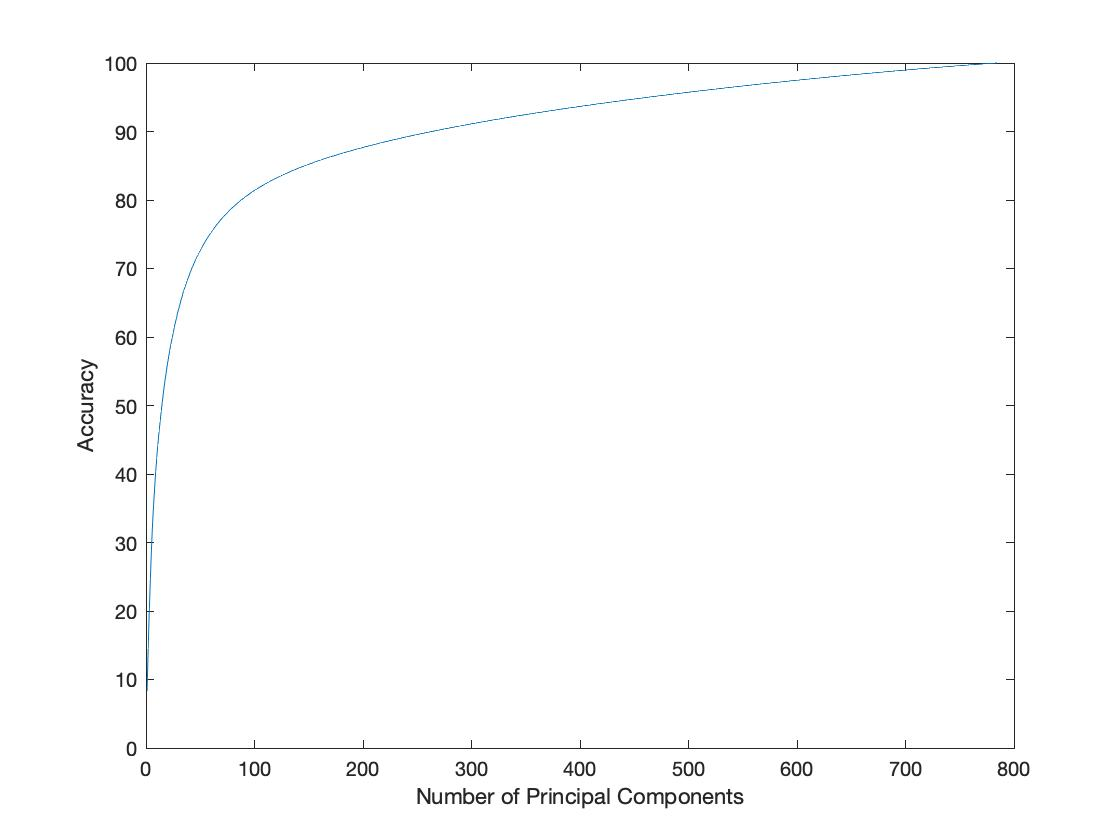
\includegraphics[width=0.7\textwidth]{3d1.jpg}
          \caption{Fractional reconstruction accuracy as a function of the number of principal components.}
          \label{fig:3d1}
        \end{figure}
    The number of principal components needed to achieve each of 90\%, 80\%, 70\%, 60\%, 50\%, 40\%, 30\%, 20\%, 10\% reconstruction accuracy:\\
    \begin{center}
      \begin{tabular}{|l|*{10}{c|}}
      \hline
      & 10\% & 20\% & 30\% & 40\% & 50\% & 60\% & 70\% & 80\% & 90\%\\ [1ex]
      \hline
      \# of principal components&2  & 4   &  6    & 9   & 15  &  25 &   43 &   88  & 264\\[2ex]
      \hline
      \end{tabular}
    \end{center}
    \clearpage
    \item For $500^{th}$ examples, please see Figure \ref{fig:3e1}. For $6000^{th}$ examples, please see Figure \ref{fig:3e2}. For $10000^{th}$ examples, please see Figure \ref{fig:3e3}.
    \begin{figure}[H]
          \centering
          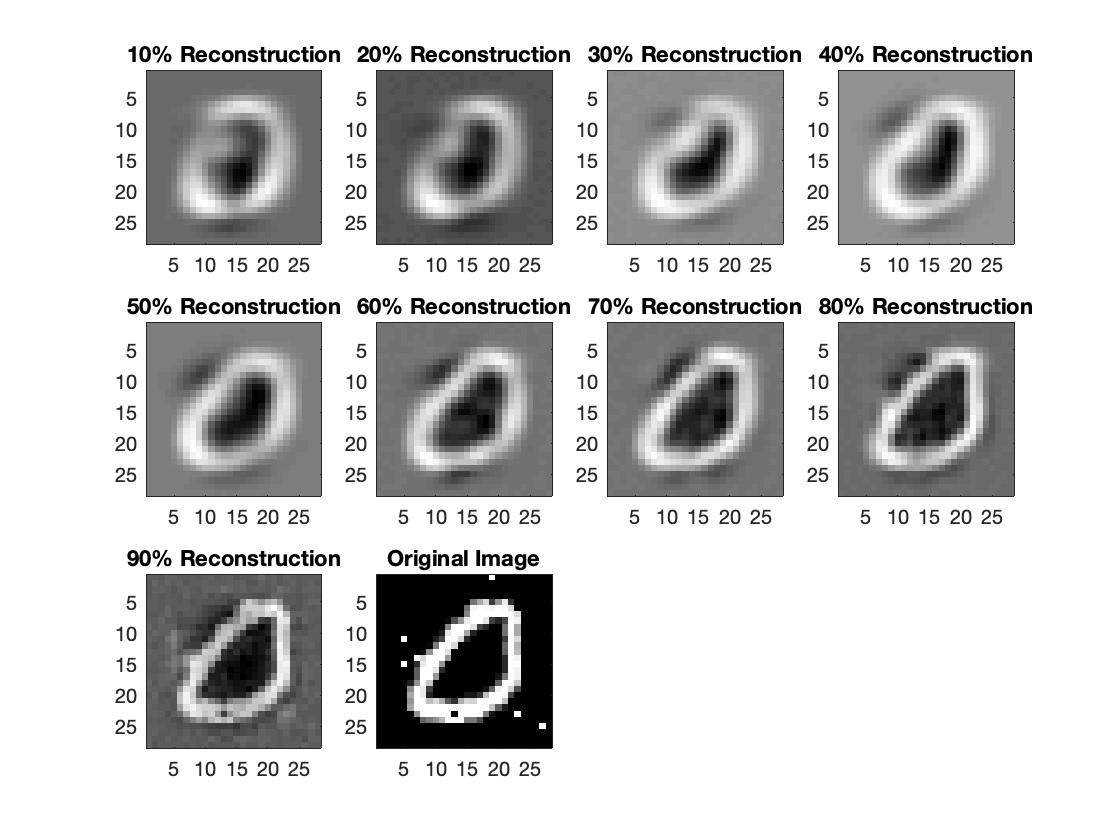
\includegraphics[width=0.7\textwidth]{3e1.jpg}
          \caption{$500^{th}$ examples}
          \label{fig:3e1}
        \end{figure}
        \begin{figure}[H]
          \centering{}
          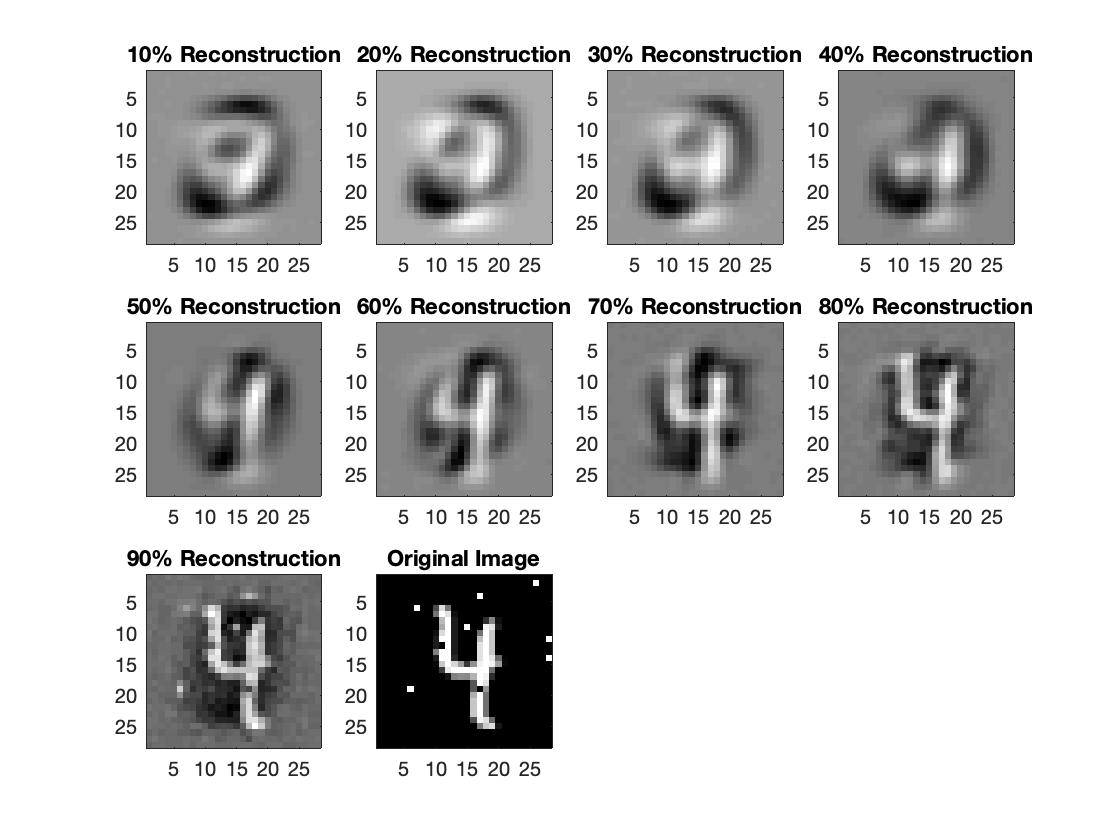
\includegraphics[width=0.7\textwidth]{3e2.jpg}
          \caption{$6000^{th}$ examples}
          \label{fig:3e2}
        \end{figure}{}
        \begin{figure}[H]
          \centering
          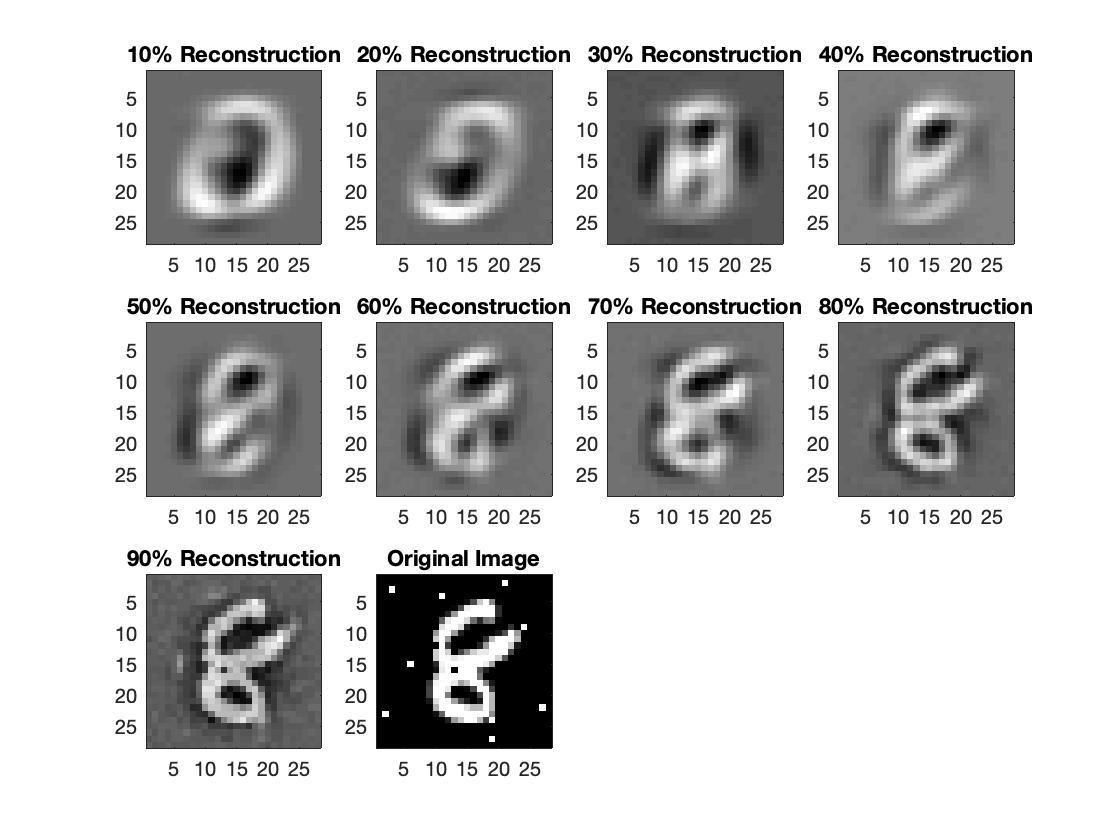
\includegraphics[width=0.7\textwidth]{3e3.jpg}
          \caption{$10000^{th}$ examples}
          \label{fig:3e3}
        \end{figure}
        \clearpage
    \item For reconstruction accuracy, please see Figure \ref{fig:3f1}.
    \begin{figure}[H]
          \centering
          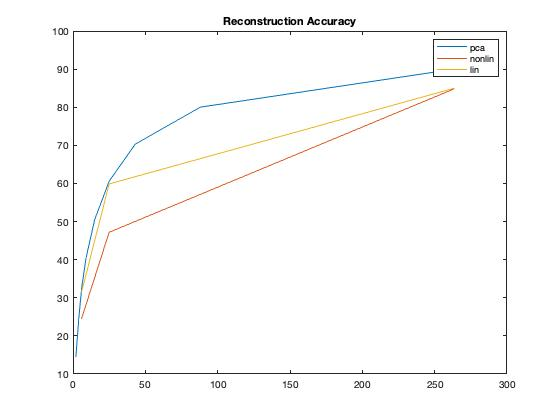
\includegraphics[width=0.7\textwidth]{3f1.jpg}
          \caption{$500^{th}$ examples}
          \label{fig:3f1}
        \end{figure}
        From the graph we can tell that PCA and autoEncoder with linear transfer functions. Both PCA and the autoEncoder works similarly. PCA is restricted to a linear map, while autoEncoders can have nonlinear enoder/decoders. A single layer autoEncoder with linear transfer function is nearly equivalent to PCA, which means that when autoEncoder has 1 hidder layer, they will have similar reconstruction accuracy, which will be higher than nonlinear function.
        \clearpage

    \item It can dependent on the number of features(neurons in input layer). Higher number of hidden layers increase order of weights and it helps to make a higher order decision boundary. Therefore increasing the number of hidden layers can decrease the reconstruction error if the autoEncoder is trained properly. As we increase the number of hidden layers then accuracy can be obtained up to great extent but neural network became complex then previous. Increasing the number of hidden layers will cause your network to overfit to the training set, that is, it will learn the training data, but it won't be able to generalize to new unseen data. There is no question to go for more and more hidden layers as the Back-Propagation algorithm will be less effective. The test set error will shoot up when you use more hidden layers though you might have got near perfect accuracy for train sets.

 \end{enumerate}
 \clearpage
 \section{Eigenvectors}
 \begin{enumerate}
    \item Since $X$ is full rank, and $rank(X) = p$, $X^TX$ is not singular. Thus we are able to write $\hat{w} = (X^TX)^{-1}X^Ty$. Since $X = U\Lambda V^T$, together with SVD, we are able to get $(X^TX)^{-1}X^T = (V\Lambda^T\Lambda V^T)^{-1}V\Lambda U^T = (V^T)^{-1}\Lambda^{-1}V^{-1}V\Lambda U^T$. Since $V^TV = I$, $\Lambda^T = \Lambda$, and $(V_P^T)^{-1} = V_P$ for thin SVD, we have $(X^TX)^{-1}X^T = V_P\Lambda_P^{-1}U_P^T$, which is the same form as $X^+$, and $X^+$ is the left inverse. In conclusion, we can say that $X^+$ with the form of $V_P\Lambda_P^{-1}U_P^T$ is the solution of the least square problem.
    \clearpage
    \item SVD of $X$ shows that $X^TX$ and $XX^T$ share the same eigenvalues: $X^TX = VD^TDV^T = VD^2V^T$ and $XX^T = UDD^TU^T = UD^2U^T$. Thus, for the right singular vector $v_i$ of $X^TX$, $X^TXv_i = \lambda_i v_i$. For the left singular vector $u_i$, $XX^Tu_i = \lambda_i u_i$. Also, both left and right singular vectors have a relation which is $X^T u_i = \sqrt{\lambda_i}u_i$. In conclusion, $v_i$ can be found by $v_i = \dfrac{X^T u_i}{\sqrt{\lambda_i}}.$
 \end{enumerate}
\end{document}
